\chapter{Les filtres numériques}

Le filtrage est un traitement qui permet de transformer  un signal. Les filtres numériques agissent sur des signaux à temps discrets c.a.d une séquence de nombres noté $\{x(n)\}$ ou $x(n)$ est la valeur du signal réel au temps $t = n.T$, $T$ étant la période d'échantillonnage.


\begin{figure}[h]
\centering
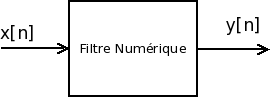
\includegraphics[scale=0.5]{digitalFilter}
\caption{Un filtre numérique}
\end{figure}

\bigskip
Un filtre numérique est entièrement définie par une équation au différence liant l'entrée $x(n)$ et la sortie $y(n)$:
\begin{equation}
y(n) = \sum_{i=0}^{N} b_{i}.x(n-i) - \sum_{i=1}^{N} a_{i}.y(n-i)
\end{equation}

\bigskip
A partir de l'équation au différence, on obtient, par transformation en Z, la fonction de transfert du filtre :
\begin{equation}
H(z) = \frac{Y(z)}{X(z)} = \frac{\sum_{i=0}^{N} b_{i}.z^{-i}}{1+\sum_{i=1}^{N} a_{i}.z^{-i}}
\end{equation}

\bigskip
Un filtre peut être spécifié par sa réponse impulsionnelle, ou son gain en fréquence ou mieux par son gabarit. 
Notons que, dans le vocabulaire du traitement des signaux, la "synthèse" consiste à trouver la valeur des coefficients $a_{n}$ et $b_{n}$ qui répond à la spécification du filtre. \\
Dans ce travail, on considère que ce calcul a déjà fait au préalable. Donc, on prend en entrée un filtre déjà définit avec les coefficients exprimés en précision "infinie". On essaiera d'obtenir une description matérielle du filtre. 


\section{Réalisation ou Structure d'un filtre}
La manière de faire les calculs dans le filtre définit la structure du filtre.
Il existe différente structure d'implémentation d'un filtre, à savoir:
\begin{itemize}
\item Forme Directe I
\item Forme Directe II : économie de stockage
\item Forme Transposée
\item Représentation d'État : utilisée en automatique
\end{itemize}
Si les calculs dans le filtre sont faits de manière exacte, il y a aucune différence sur les structures.
Mais en précision finie, le résultat dépend beaucoup de la structure utilisé.
\begin{itemize}
\item les coefficients ne sont pas exactes
\item les calculs ne sont pas exactes
\end{itemize}

\section{La Forme implicite - S.I.F}
[Hilaire06] [Benoit - page 27] [FWRUserGuide - page 10]
La représentation d'état est très utilisée pour étudier un filtre, mais elle n'est pas complète et a quelques limitations :
\begin{itemize}
\item difficile d'analyser l'effet d'arrondi sur un coefficient particulier
\item Absence de variable intermédiaire utile pour l'expression de certaines réalisations
\end{itemize}

\bigskip
Avantages:
\begin{itemize}
\item analyse facile des effets de la précision finie
\item description de haut niveau plus généralisé et plus précis
\end{itemize}


